%! TeX root = master.tex
% !TEX program = lualatex

\lecture{4}{10-03-26}{Linear Models for Classification (Multi-class classification)}{}

\subsection{Classification evaluation}
\begin{wrapfigure}{r}{0.3\linewidth}
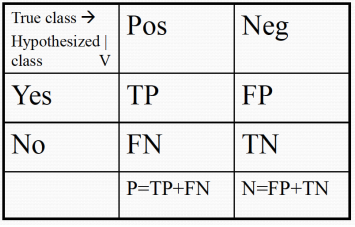
\includegraphics[width=\linewidth]{images/img_20260311_212913.png}
\end{wrapfigure}
For binary case we could use confusion matrix:\\
TP: True positive (number of samples correctly classified as positive)\\
FP: False positive (number of samples incorrectly classified as positive)\\
TN: True negative (number of samples correctly classified as negative)\\
FN: False negative (number of samples incorrectly classified as negative)\\
P: Total number of positive samples\\
N: Total number of negative samples\\

\begin{definition}[Accuracy]
Percentage of correctly classified samples \[
  Acc = \frac{TP + TN}{P + N}
\]
\end{definition}

However, the accuracy doesn't give the information about the behavior of a model, in fact models with same accuracy could have a totally different behavior(e.g, one performing poorly on positive recogniton and well on negative one and the other one the total contrary). \\
Thus we could use other metrics in complement: 

\begin{definition}[Precision]
Percentage of samples classified as positives that
are truly positives \[
  Precision = \frac{TP}{TP + FP}
\]
\end{definition}

\begin{definition}[Recall]
Percentage of positive samples that are correctly
classified as positives
  \[
    Recall = \frac{TP}{P}
  \]
\end{definition}

But, still two classifiers with the same precision and recall could have a very different behavior as before (checking for accuracy could clearly show this), so we could too look for : 
\begin{definition}[False positive rate]
  Percentage of negative samples that are incorrectly classified as positives
  \[
    FP \text{ } rate = \frac{FP}{N}
  \]
\end{definition}

\begin{definition}[F1 score]
Single number that combines precision and recall (good for unbalance data)
  \[
    F1 = 2 \cdot \frac{Precision \cdot Recall}{Precision + Recall}
  \]
\end{definition}

\subsubsection{ROC curves}
\begin{wrapfigure}{r}{0.5\linewidth}
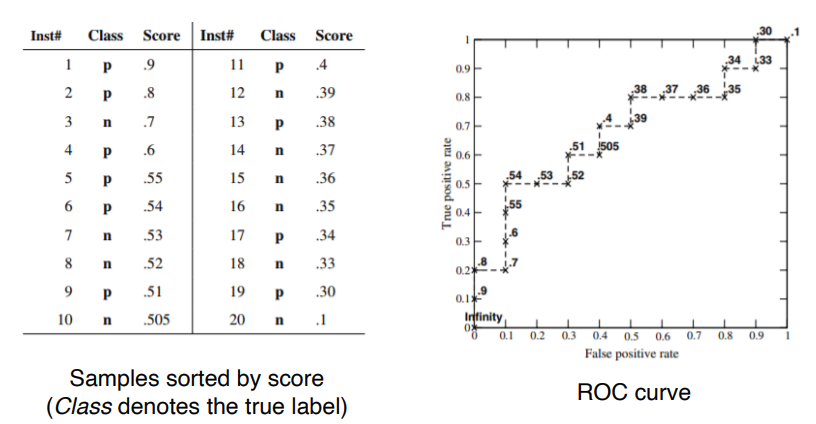
\includegraphics[width=\linewidth]{images/img_20260311_214205.png}
\end{wrapfigure}
Many classifiers output a score/confidence for their predictions (e.g., $\hat{y}$ is a continuous value between 0 and 1 in logistic regression).  \\
The decision between positive and negative can be computed by thresholding this score:
\[
  \text{label}_i = 1 \text{ if } \hat{y_i} \geq \tau
\]
where $\tau$ is a given threshold

The Receiver Operating Characteristic (ROC) curve plots the true positive rate (recall) as a function of the false positive rate, obtained by varying the score threshold. \\
This model give a score(probability) to each observation(here Inst#) and make the threshold vary, then compute the TP and FP rate, and plot the curves. \\ 
A good model as a plot near the top left corner (meaning that the TP rate is high and the FP rate low) as we mesure the quality of the model with the Area under the curve \textbf{(AUC)}(goes from 0 to 1), 1.0 that the model is perfect, 0.5 is the result if the model makes random predictions, and less is worse than randomness. 

\subsection{From binary to multi-class classification}
What if we have more than two classes? How our three linear models can handle this scenario ?

\subsection{Decision boundaries: General Definition}
\begin{wrapfigure}{r}{0.3\linewidth}
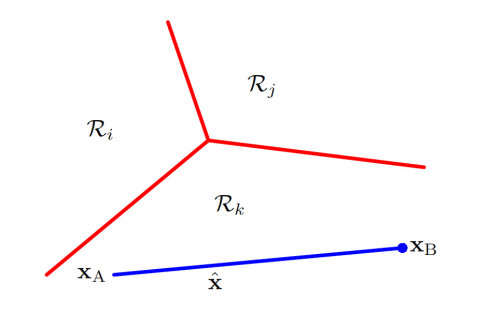
\includegraphics[width=\linewidth]{images/img_20260311_222244.png}
\end{wrapfigure}

First let's update our knowledge on decision boundaries, as here we are not anymore treating binary label. \\ 
The decision boundary between two classes $k$ and $j$ is defined as the set of points  \textbf{x} such that \[
 \hat{y}^{\left(k\right)}(x) = \hat{y}^{\left(j\right)}(x)
\]\\
This corresponds to the $(D - 1)-$dimensional hyperplane. \\
The decision regions are \textbf{singly-connected and convex} (any point $\hat{x}$ between two points $x_A$ and $x_B$ in the same region (e.g, k) will also be in the same region)

Decision boundaries for C = 4 and C = 5 classes. 

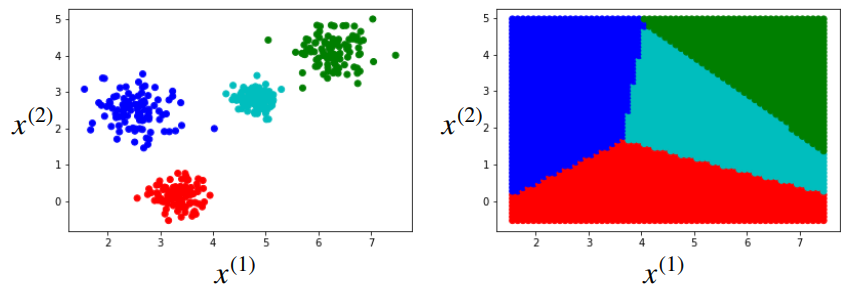
\includegraphics[width=0.5\linewidth]{images/img_20260311_222448.png}
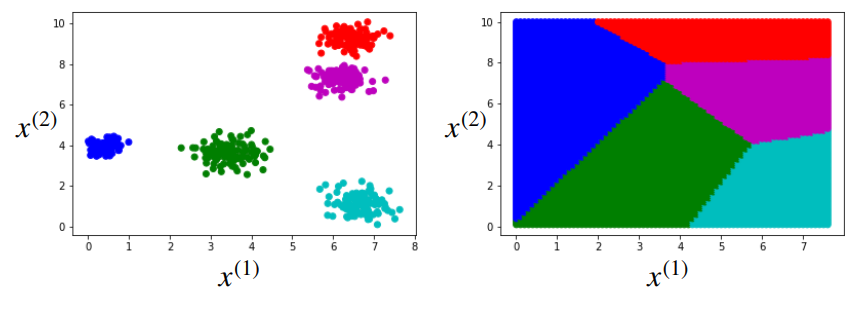
\includegraphics[width=0.5\linewidth]{images/img_20260311_222503.png}

\subsection{Classification evaluation for Multi-class}

\begin{wrapfigure}{r}{0.4\linewidth}
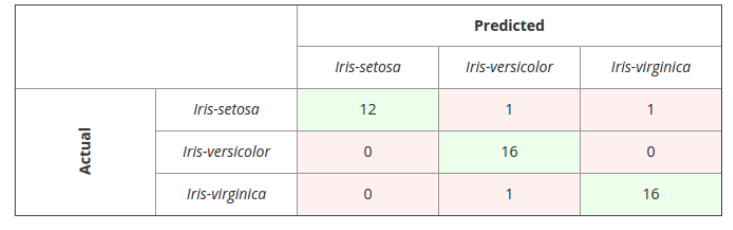
\includegraphics[width=\linewidth]{images/img_20260311_232206.png}
\end{wrapfigure}
Confusion matrix for multi-class case.\\
\textbf{Accuracy} : A global accuracy can be obtained by summing the correct predictions for all
classes (diagonal values of the confusion matrix), and dividing this by the
total number of samples (sum of all entries in the confusion matrix). \\
\textbf{Precision, recall, FP-rate and F1-score}:
The simplest approach to handling these metrics is to compute them for
each individual class, and then average over the classes.\\
In this case, each individual class is in turn considered as the “positive” class
while the others act as the “negative” class.\\
This does not account for class imbalance (some classes may have many
more samples than others; more about this in a future lecture).\\
This can be handled by weighting the metric for each class by a value
depending on the proportion of samples from that class.

\subsection{Least-square classification}
The most common approach to modeling a multi-class problem
consists of encoding the class label as a vector with a single 1
at the index corresponding to the category and 0s elsewhere. \\
\textbf{e.g.} in a 5-class problem, a sample in class 2 is represented as:
\[
  y = \begin{pmatrix} 0 \\ 1 \\ 0 \\ 0 \\ 0
  \end{pmatrix}
\] This is referred as \textbf{one-hot-encoding}.  \\ 
As this is similar to making the model output multiple (as for multi-output regression), we therefore again use a matrix \textbf{W} $\in \mathbb{R}^{\left(D+1\right)\times C}$, s.t \[
  \hat{y_i} = W^T x_i = \begin{pmatrix} w_\left(1\right)^T \\ w_\left(2\right)^T \\ \vdots \\ w_\left(C\right)^T
  \end{pmatrix} x_i 
\]
where each $w_\left(j\right)$ is a $(D + 1)-$dimensional vector, used to predict one output dimension, i.e., the \textbf{score} for one class.
\subsubsection{Training}
We can then write training as \[
  min_w \sum_{i=1}^{N}\left\|W^Tx_i - y_i\right\|^2 
\]
where each $y_i$ is now a $C-$dimensional vector with a single one at the index corresponding to the class label and zeroes everywhere else.
\subsubsection{Solution}
The inputs and the outputs are two matrices: 
\[
  X = \begin{pmatrix}
   x_i^T \\ x_2^T \\ \vdots \\ x_N^T  
  \end{pmatrix}
  \in \mathbb{R}^{N \times \left(D+1\right)} \quad Y = \begin{pmatrix}
   y_i^T \\ y_2^T \\ \vdots \\ y_N^T  
 \end{pmatrix} \in \mathbb{R}^{N \times C}
\]
$X$ = data \quad $Y$ = True classes \\ $N$ = number of samples \quad $D$ = number of features (+1 for bias) \quad $C$ = number of classes \\
Then, the solution has the same form as in the regression case (obtained by zeroing out the gradient w.r.t. W), i.e., \[
  W^* = (X^TX)^{-1}X^TY = X^{\dagger}Y
\]
$W$ = weight matrix (e.g, $W = [W_0, W_1]$, \quad $W_0, W_1 _$ weight classes 0 and 1)
\subsubsection{Prediction}
Given the optimal parameters, the prediction for a new sample is computed as \[
  \hat{y} = (W^*)^Tx 
\]\\
The sample is then assigned to class k if 
\[
\hat{y}^{\left(k\right)} > \hat{y}^{\left(j\right)}, \quad \forall j \neq k
\]
In other words the final label k is obtained as \[
  k = \operatorname*{argmax}_j \hat{y}^{\left(j\right)}
\]
That is, the label is the index (position) of the maximum value in the vector $\hat{y}$
\\
E.g: if we have \[
  \hat{y} = \begin{pmatrix} \hat{y}^{\left(1\right)} \\ \hat{y}^{\left(2\right)} \\ \hat{y}^{\left(3\right)}\end{pmatrix} = \begin{pmatrix} 2.3 \\ 0.7 \\ -1.5\end{pmatrix}
\] here the $\operatorname*{argmax}_j$(biggest score) is 2.3, so the label predicted is the label 1.
\\

(boundary where $\hat{y}_i$ = $\hat{y}_k$ (for 2 different classes))
Example of success and failure case of 2D inputs and 3 classes least-square classification:
\begin{center}
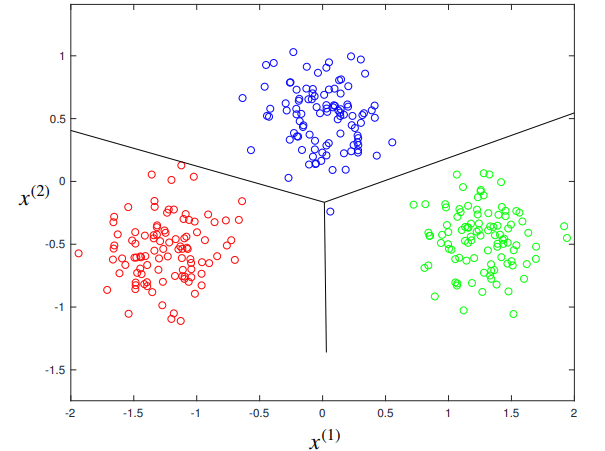
\includegraphics[width=0.4\linewidth]{images/img_20260311_222715.png}
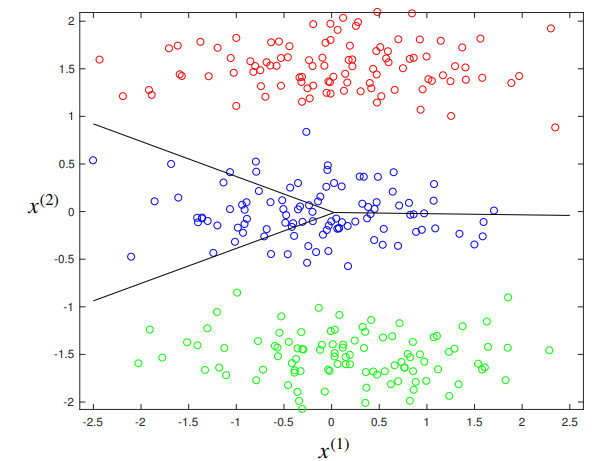
\includegraphics[width=0.4\linewidth]{images/img_20260311_222727.png}
\end{center}

\subsubsection{Drawbacks}
As in the binary case, the multi-class least-square classification suffer from outliers, because it tries to minimize the distance (regression). So we need an other model like the logistic regression one but for multi-class: \textbf{Multi-class logistic regression} :O !!

\subsection{Multi-class logistic regression}
We still use the one-hot enconding to represent multi-class labels. \\
We again need to use a matrix \textbf{W} $\in \mathbb{R}^{\left(D+1\right)\times C}$ to represent the model parameters. \\
But now, the probability for a class $k$ is given by the \textbf{softmax} function (takes scores and transforms them into probabilities) \[
    \hat{y}^{\left(k\right)}(x) = \frac{\exp(w_{\left(k\right)}^Tx)}{\sum_{j=1}^{C}\exp(w_{\left(j\right)}^Tx)}
  \]
\\
The empirical risk can then be derived from the multi-class version of the cross entropy, which yields \[
  R(W) = - \sum_{i=1}^{N}\sum_{k=1}^{C}y_i^{\left(k\right)}\ln \hat{y}_i^{\left(k\right)} = - \sum_{i=1}^{N}\ln\hat{y}_i^{\text{(true class of i)}}
\](i \to go through the samples, k \to go through the classes) 
\\
As in the binary case :
\begin{itemize}
  \item a single $y_i^{\left(k\right)}$ is 1 for every sample $i$, so we really have one term per training sample. (as if sample $k$ belongs to class $i$ then only the term for this class/label stay in the sum (other are 0))
  \item training is done by minimizing this empirical risk using gradient descent
\end{itemize}
\subsubsection{Gradient}

The gradient descent is the same algorithm as for the muti-outputs binary case, the only difference is that the parameters are shaped as a matrix \textbf{W} $\in \mathbb{R}^{\left(D+1\right) \times C}$, not a vector anymore :\\
\textbf{Algorithm - gradient descent}
\begin{itemize}
  \item 1. Initialize $W_0$ (e.g, randomly)
  \item 2. While not converged \implies  update $ W_k \leftarrow W_{k-1} - \eta \nabla_W R(W_{k-1})$
\end{itemize}
Thus the gradient will also be a matrix 

\[
\nabla_WR(W_{k-1}) = \sum_{i=1}^{N}x_i(\hat{y}_i - y_i)^T \quad  \in \mathbb{R}^{\left(D+1\right) \times C}
\]

\subsubsection{Prediction}

At test time, given a new input sample \textbf{x}, the probability for any class $k$ is computed via the softmax function as \[
  \hat{y}^{\left(k\right)}(x) = \frac{\exp((w_{\left(k\right)}^*)^Tx)}{\sum_{j=1}^{C}exp((w_{\left(j\right)}^*)^Tx) } 
\]
The final class label is then predicted as \[
  k = \operatorname*{argmax}_j \hat{y}^{\left(j\right)}(x)
\]

That is, as in least-square classification, the label is the
index (position) of the maximum value in the vector $\hat{y}$.

\subsubsection{Example}
2D inputs, 3 classes: Logistic regresison results \\
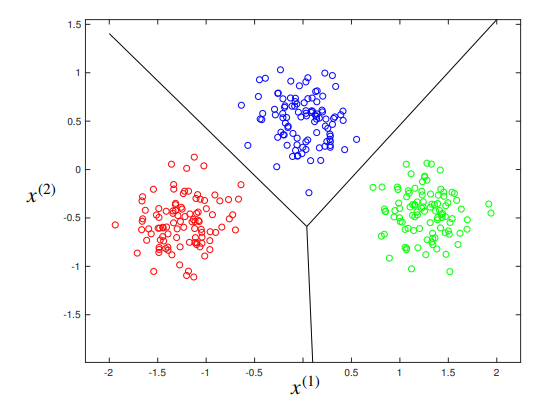
\includegraphics[width=0.4\linewidth]{images/img_20260311_231537.png}
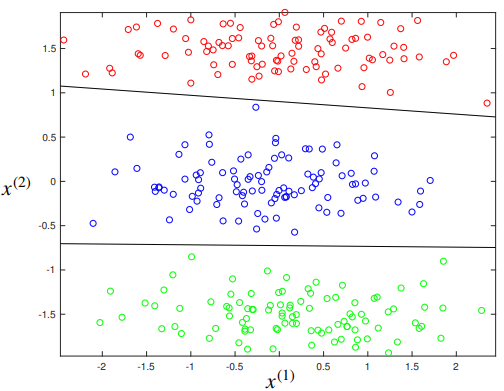
\includegraphics[width=0.4\linewidth]{images/img_20260311_231544.png}


\subsection{Dealing with multiple classes}
SVM cannot be extended to the multi-class scenario. \\
Instead one can use several binary classifier E.g, one-vs-rest or one-vs-one (however leaves ambiguities and inconsistencies (a sample can be classified being from more that one class at a time))
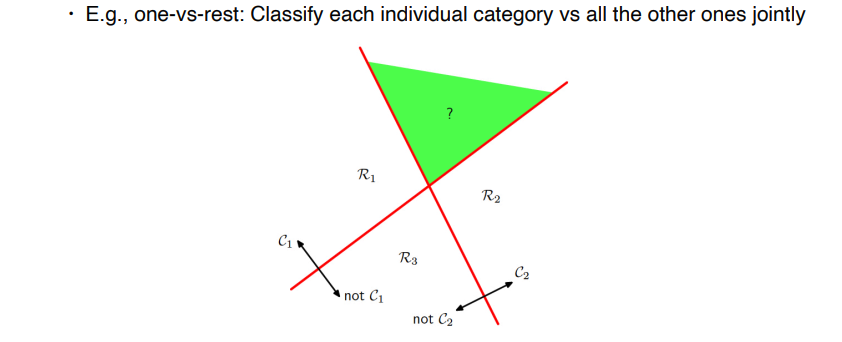
\includegraphics[width=0.5\linewidth]{images/img_20260311_234308.png}
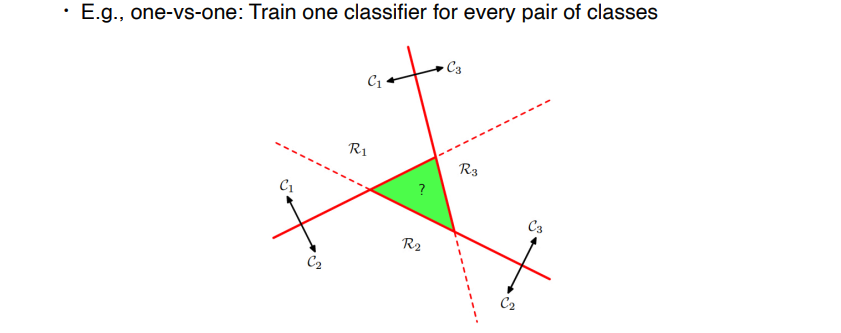
\includegraphics[width=0.5\linewidth]{images/img_20260311_234320.png}

\subsection{Comparing linear classifiers}
We have now seen 3 different linear(multi-class) classifiers: Least-square classification, Logistic regression, SVM. \\
In practice, one almost never uses the least-square one (only for pedagogiqual standpoint).\\
Depending on the data to classify, we may use Logistic regression or SVM as they are both better than the other one depending of the data.

\subsection{Recap - and new challenge}
Linear regression : Fit a linear model to the observations\\
Binary linear classification: Use a linear model to separate the positive and negative samples\\
Multi-class linear classification: Use a linear model to separate the classes, via a one-hot encoding of the label

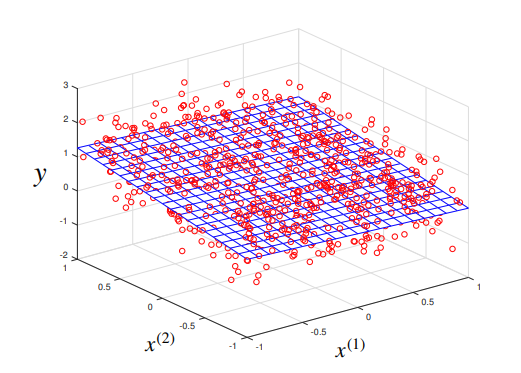
\includegraphics[width=0.3\linewidth]{images/img_20260311_234835.png}
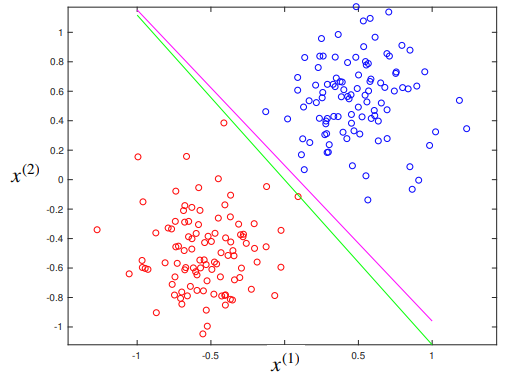
\includegraphics[width=0.3\linewidth]{images/img_20260311_234923.png}
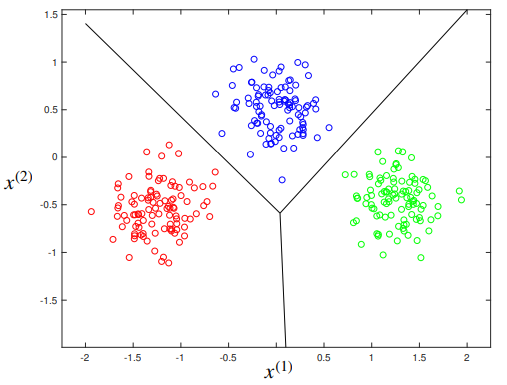
\includegraphics[width=0.3\linewidth]{images/img_20260311_234938.png}
\\
Unfortunately, no linear model can directly fit non linear data (we will go from linear to non linear model).
